% 
% ENGR 1120 021  
% Tristan Hill - FAll 2016 (first term) 
% Lab 2 - Basic User Input and Output 
%       - fprintf and input 
% The Ideal Gas Law 
 

% Document settings
\documentclass[11pt]{article}
\usepackage[margin=1in]{geometry}
\usepackage[pdftex]{graphicx}
\usepackage{multirow}
\usepackage{setspace}
\usepackage{hyperref}
\usepackage{color,soul}
\usepackage{fancyvrb}
\usepackage{framed}
\usepackage{wasysym}
\usepackage{multicol}

\pagestyle{plain}
\setlength\parindent{0pt}
\hypersetup{
    bookmarks=true,         % show bookmarks bar?
    unicode=false,          % non-Latin characters in Acrobat’s bookmarks
    pdftoolbar=true,        % show Acrobat’s toolbar?
    pdfmenubar=true,        % show Acrobat’s menu?
    pdffitwindow=false,     % window fit to page when opened
    pdfstartview={FitH},    % fits the width of the page to the window
    pdftitle={My title},    % title
    pdfauthor={Author},     % author
    pdfsubject={Subject},   % subject of the document
    pdfcreator={Creator},   % creator of the document
    pdfproducer={Producer}, % producer of the document
    pdfkeywords={keyword1} {key2} {key3}, % list of keywords
    pdfnewwindow=true,      % links in new window
    colorlinks=true,       % false: boxed links; true: colored links
    linkcolor=red,          % color of internal links (change box color with linkbordercolor)
    citecolor=green,        % color of links to bibliography
    filecolor=magenta,      % color of file links
    urlcolor=blue           % color of external links
}

% assignment number 
\newcommand{\NUM}{2} 
\newcommand{\VSpaceSize}{2mm} 
\newcommand{\HSpaceSize}{2mm} 

\definecolor{mygray}{rgb}{.6, .6, .6}

\setulcolor{red} 
\setstcolor{green} 
\sethlcolor{mygray} 

\begin{document}

	\textbf{\LARGE Intro to Programming with Python -  Summer 2023} \\\\
	\textbf{\LARGE Tutorial \NUM: Command Window Output} \\\\
	\textbf{\LARGE Chemistry: The Ideal Gas Law} \\
	
	
	\begin{description}
        \vspace{3mm}
		\item [\textbf{ \Large Overview}] \textbf{ \Large :}\\
			You will practice basic calculations and add formatted output to a Python program. The {\it print} function will be used to display formatted strings to the command window. You will complete a basic, but fundamental chemistry calculation. The inputs are typed in your program and the program will output the results to the command window. \\
 
        \item [\textbf{ \Large What is a Mole?}] \textbf{ \Large :}\\   
            The mole is a unit of measurement used in chemistry to express amounts of a chemical substance, defined as the amount of any substance that contains as many elementary entities (e.g., atoms, molecules, ions, electrons) as there are atoms in 12 grams of pure carbon-12. This number is called {\it Avogadro's Constant} and has a value of $6.0221\times10^{23}$. \\
            
        \item [\textbf{ \Large The Ideal Gas Law}] \textbf{ \Large :}\\  
            The following equations describe the behavior of a gas in the form of the temperature, pressure, volume and mass relation. The equation to find the force on the piston is also given. You will use them in your program. \\

             \scalebox{1.3}{$PV=nRT$}   \hspace{15mm}    \scalebox{1.5}{$n=m/M$} \hspace{15mm} \scalebox{1.5}{$P = F/A $} 
                                 
            
            where,\\
            
            \begin{multicols}{2}
            
            \begin{tabular}{lll}
            x &position &($m$)   \\
            F &force    &($N$)   \\
            V &volume   &($m^3$) \\        
            n &number of moles &($mols$) \\   
            m & mass of gas&($kg$)      \\ 
            \\
            A=100 &area     &($cm^2$)  \\
            P=300 &pressure &($kPa$) \\ 
            T=325 & temperature &($K$) \\\\ 
            M=28.97 & molecular mass of air &($\frac{g}{mol}$)       \\\\ 
            R=8.314 & ideal gas constant &($\frac{Pa\hspace{1mm}m^3}{mol\hspace{1mm}K}$)\\ 
            \end{tabular}\\

            
            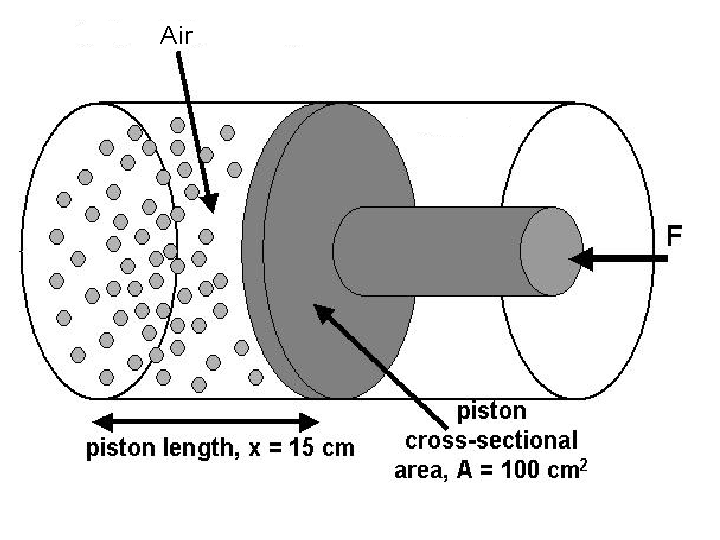
\includegraphics[scale=.35]{ideal_gas_law_fig1.png} \\    
            \end{multicols}
               1($kPa$)=1000($Pa$)\\
               1($Pa$)=1($\frac{N}{m^2}$)
\newpage


       
        \item [\textbf{ \Large Assignment}] \textbf{ \Large :}
            Your program should do the following:\\\\
            \begin{enumerate}
            \item
            {\bf R}, {\bf M}, {\bf T}, {\bf P}, and {\bf A}, are constants. {\it Hardcode} these in your program. \\
            \item
            Consider the piston at position  {\bf x=15 cm}. Calculate the force, {\bf F} required to hold the piston at the current position..\\	
            \item
            Calculate the remaing quantities {\bf V}, {\bf n}, and {\bf m}.\\ 
            \item
            Output the 4 results to the command window in the {\it base S.I. units}. \\
            \item
            Consider the piston has moved to {\bf x=10 cm} and the temperature, T stays constant. Calculate and output the quantities that have changed. Do not output the quantities that have \underline{not} changed.\\\\  
             
        	\end{enumerate}

\item [\textbf{Submission }]\textbf{:} \\
			\begin{itemize}
				\item Your program needs a proper {\it Header} or title block on it. Please see this discussion in the notes for details.\\
				\item Your script file needs to be named properly. Please see the {\it naming convention} document on ilearn. \\
				\item Submit your file on ilearn in the {\bf Laboratory Assignment \NUM \hspace{2mm}Folder}. You can resubmitt as many times as you would like but please wait at least 2 minutes between submissions. Your latest submission will be the only one graded.

			\end{itemize}


	\end{description}
 
\end{document}



